\documentclass{standalone}
\usepackage{tikz}
\usetikzlibrary{shapes.geometric, arrows}

\definecolor{mycolor}{RGB}{0, 153, 255}
\tikzstyle{process} = [rectangle, rounded corners,
                       minimum width=2cm, minimum height=1cm,
                       text centered, draw=black, fill=mycolor,
                       text=white, line width=0.3mm]

\tikzstyle{arrow} = [thick,->,>=stealth]

\begin{document}
    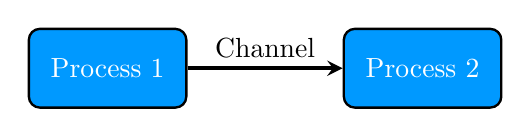
\begin{tikzpicture}[node distance=2cm]
        
        \node (Process1) [process] {Process 1};
        
        \node (Process2) [process, right of = Process1, xshift=2cm] {Process 2};
        
        \draw [arrow, line width=0.5mm] (Process1) -- node[anchor=south] {Channel} (Process2);
    
    \end{tikzpicture}
\end{document}
